COLING 2025 is thrilled to offer attendees a range of exciting social events and excursions in Abu Dhabi, providing the perfect mix of culture, history, and adventure. As part of the full conference registration, the Social Excursion Dinner in the Desert is included, and additional excursions are available for those interested in exploring the region in greater depth.\\

\noindent{\textbf{Social Excursion Dinner in the Desert}}\\
 Date: \textbf{January 23, 19:00 - 22:30}\\
 Details: Enjoy an unforgettable BBQ buffet under the stars in the desert, accompanied by refreshing beverages. This event is included with your full conference registration and promises to be a highlight of your COLING 2025 experience.\\

\noindent{\textbf {Excursion Options (Included for Full Conference Registration)}}\\ 
\noindent{We are excited to offer 3 unique excursion options this year, each designed to cater to different interests:}
\begin{enumerate}[noitemsep]
  \item For History Enthusiasts:
  \begin{itemize}[noitemsep]
    \item Abrahamic House \& Louvre Abu Dhabi: Explore the rich cultural heritage of the region with a visit to the Abrahamic House, a symbol of unity, and the world-renowned Louvre Abu Dhabi, showcasing masterpieces from diverse cultures and historical periods.
  \end{itemize}
  \item For Architecture and Culture Lovers:
  \begin{itemize}[noitemsep]
    \item Grand Mosque \& Qasr Al Watan (Presidential Palace): Discover the awe-inspiring beauty of the Sheikh Zayed Grand Mosque, followed by a visit to the magnificent Qasr Al Watan, the Presidential Palace, where you will experience the opulence and grandeur of Abu Dhabi's heritage.
  \end{itemize}
  \item For Adventure Seekers:
  \begin{itemize}[noitemsep]
    \item Dune Bashing, Sand Surfing, and Camel Riding: For those seeking adrenaline, embark on an exciting adventure through the desert with dune bashing and sand surfing, followed by a traditional camel ride. The excursion concludes with the unforgettable Social Excursion Dinner in the Desert.
  \end{itemize}
\end{enumerate}
\noindent\hrulefill\\
\noindent{Ticket Pricing for Additional Guests}
\begin{itemize}[noitemsep]
\item Social Event Ticket (Additional Guest): \$150
\item Social Event Ticket (Under 10): \$75
\item Social Event Ticket (Exhibitor): \$150
\end{itemize}
Tickets for these exciting excursions and social events can be purchased on-site. Be sure to book early, as spots are limited!
\newpage
\subsection{Social Excursion Option 1: Grand Mosque and Presidential Palace Afternoon Tour}
\noindent{\textbf{1. Sheikh Zayed Grand Mosque}}\\
\begin{figure}[h!]
  \centering
      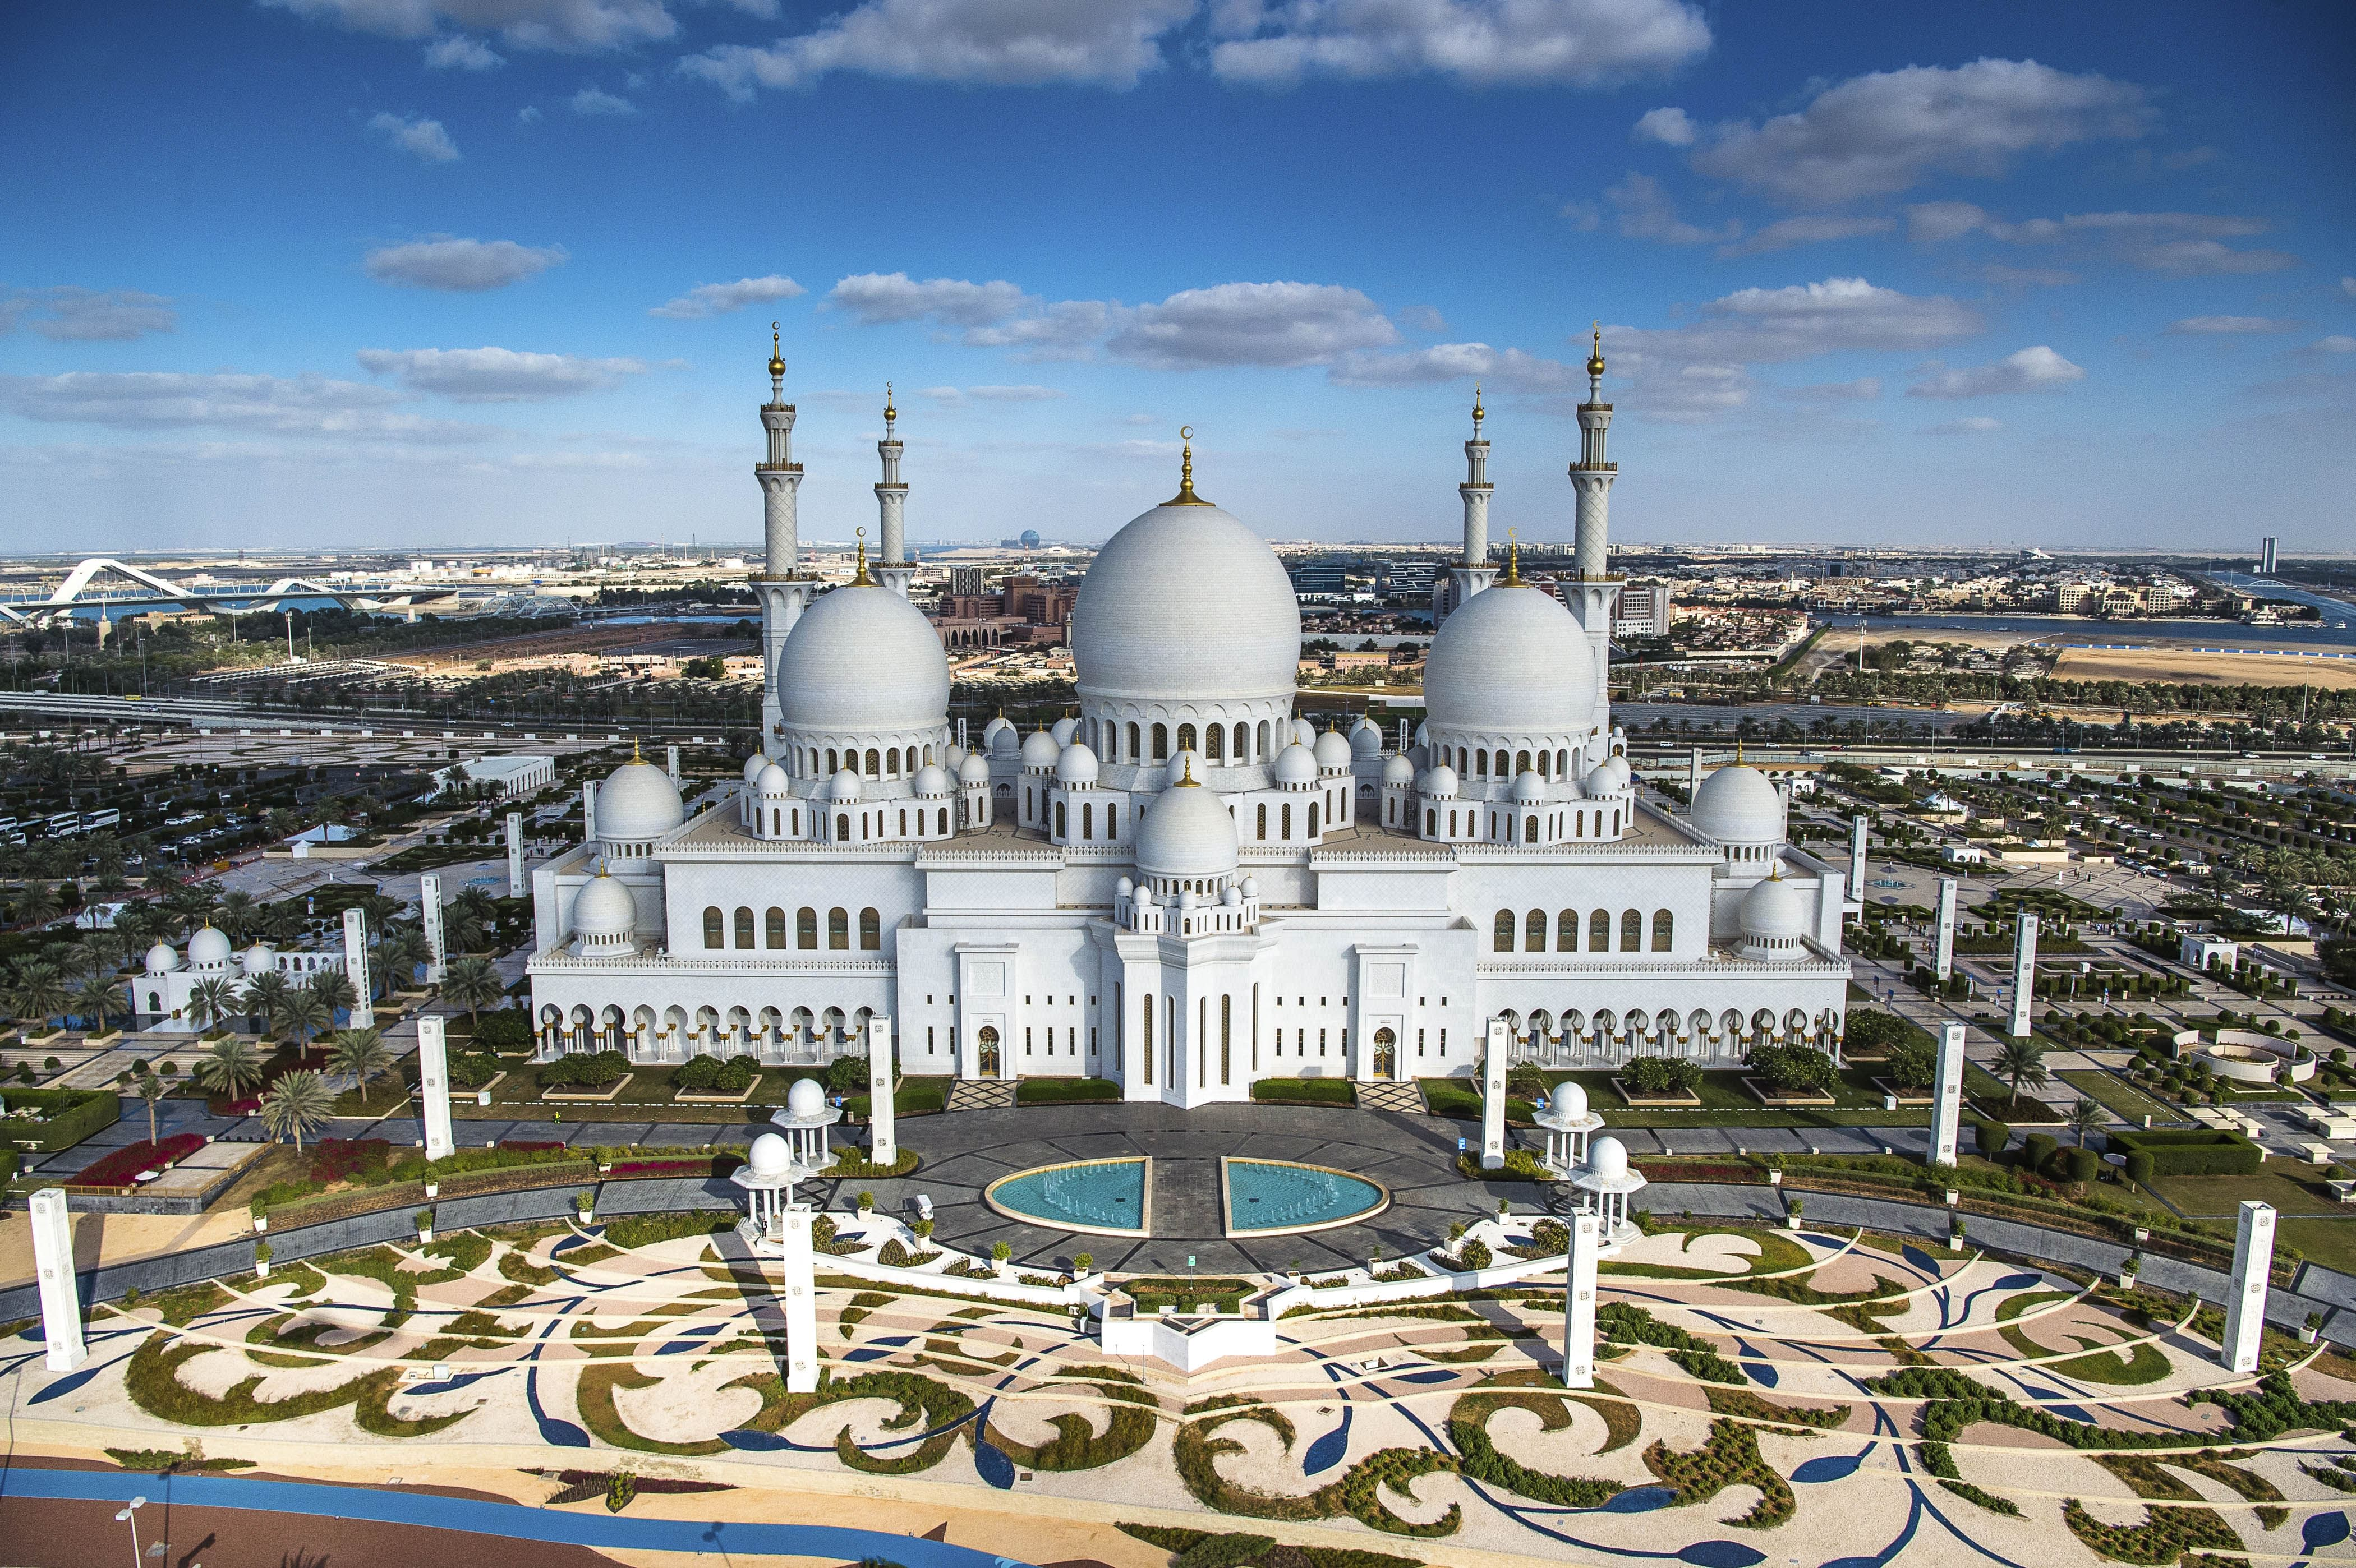
\includegraphics[width=0.45\linewidth]{examples/handbook_coling25/social_event/images/grand_mosque.png}
\end{figure}
\noindent{The day begins with a visit to the Sheikh Zayed Grand Mosque, one of the largest and most beautiful mosques in the world. This architectural marvel is known for its stunning white marble exterior, grand prayer halls, and impressive minarets. Visitors will have the opportunity to explore the mosque’s intricate interiors, including the largest hand-knotted carpet in the world, crystal chandeliers, and the peaceful courtyards. The mosque can accommodate over 40,000 worshippers and is a masterpiece of Islamic architecture, blending traditional and modern design elements.
}\\
\noindent{Key highlights}
\begin{itemize}[noitemsep]
  \item Majestic prayer halls
  \item Grand chandeliers and domes
  \item Expansive courtyards and reflective pools
  \item Impressive Islamic calligraphy and marble work
\end{itemize}

\noindent{\textbf{2. Qasr Al Watan (The Presidential Palace)}}\\
\begin{figure}[h!]
  \centering
  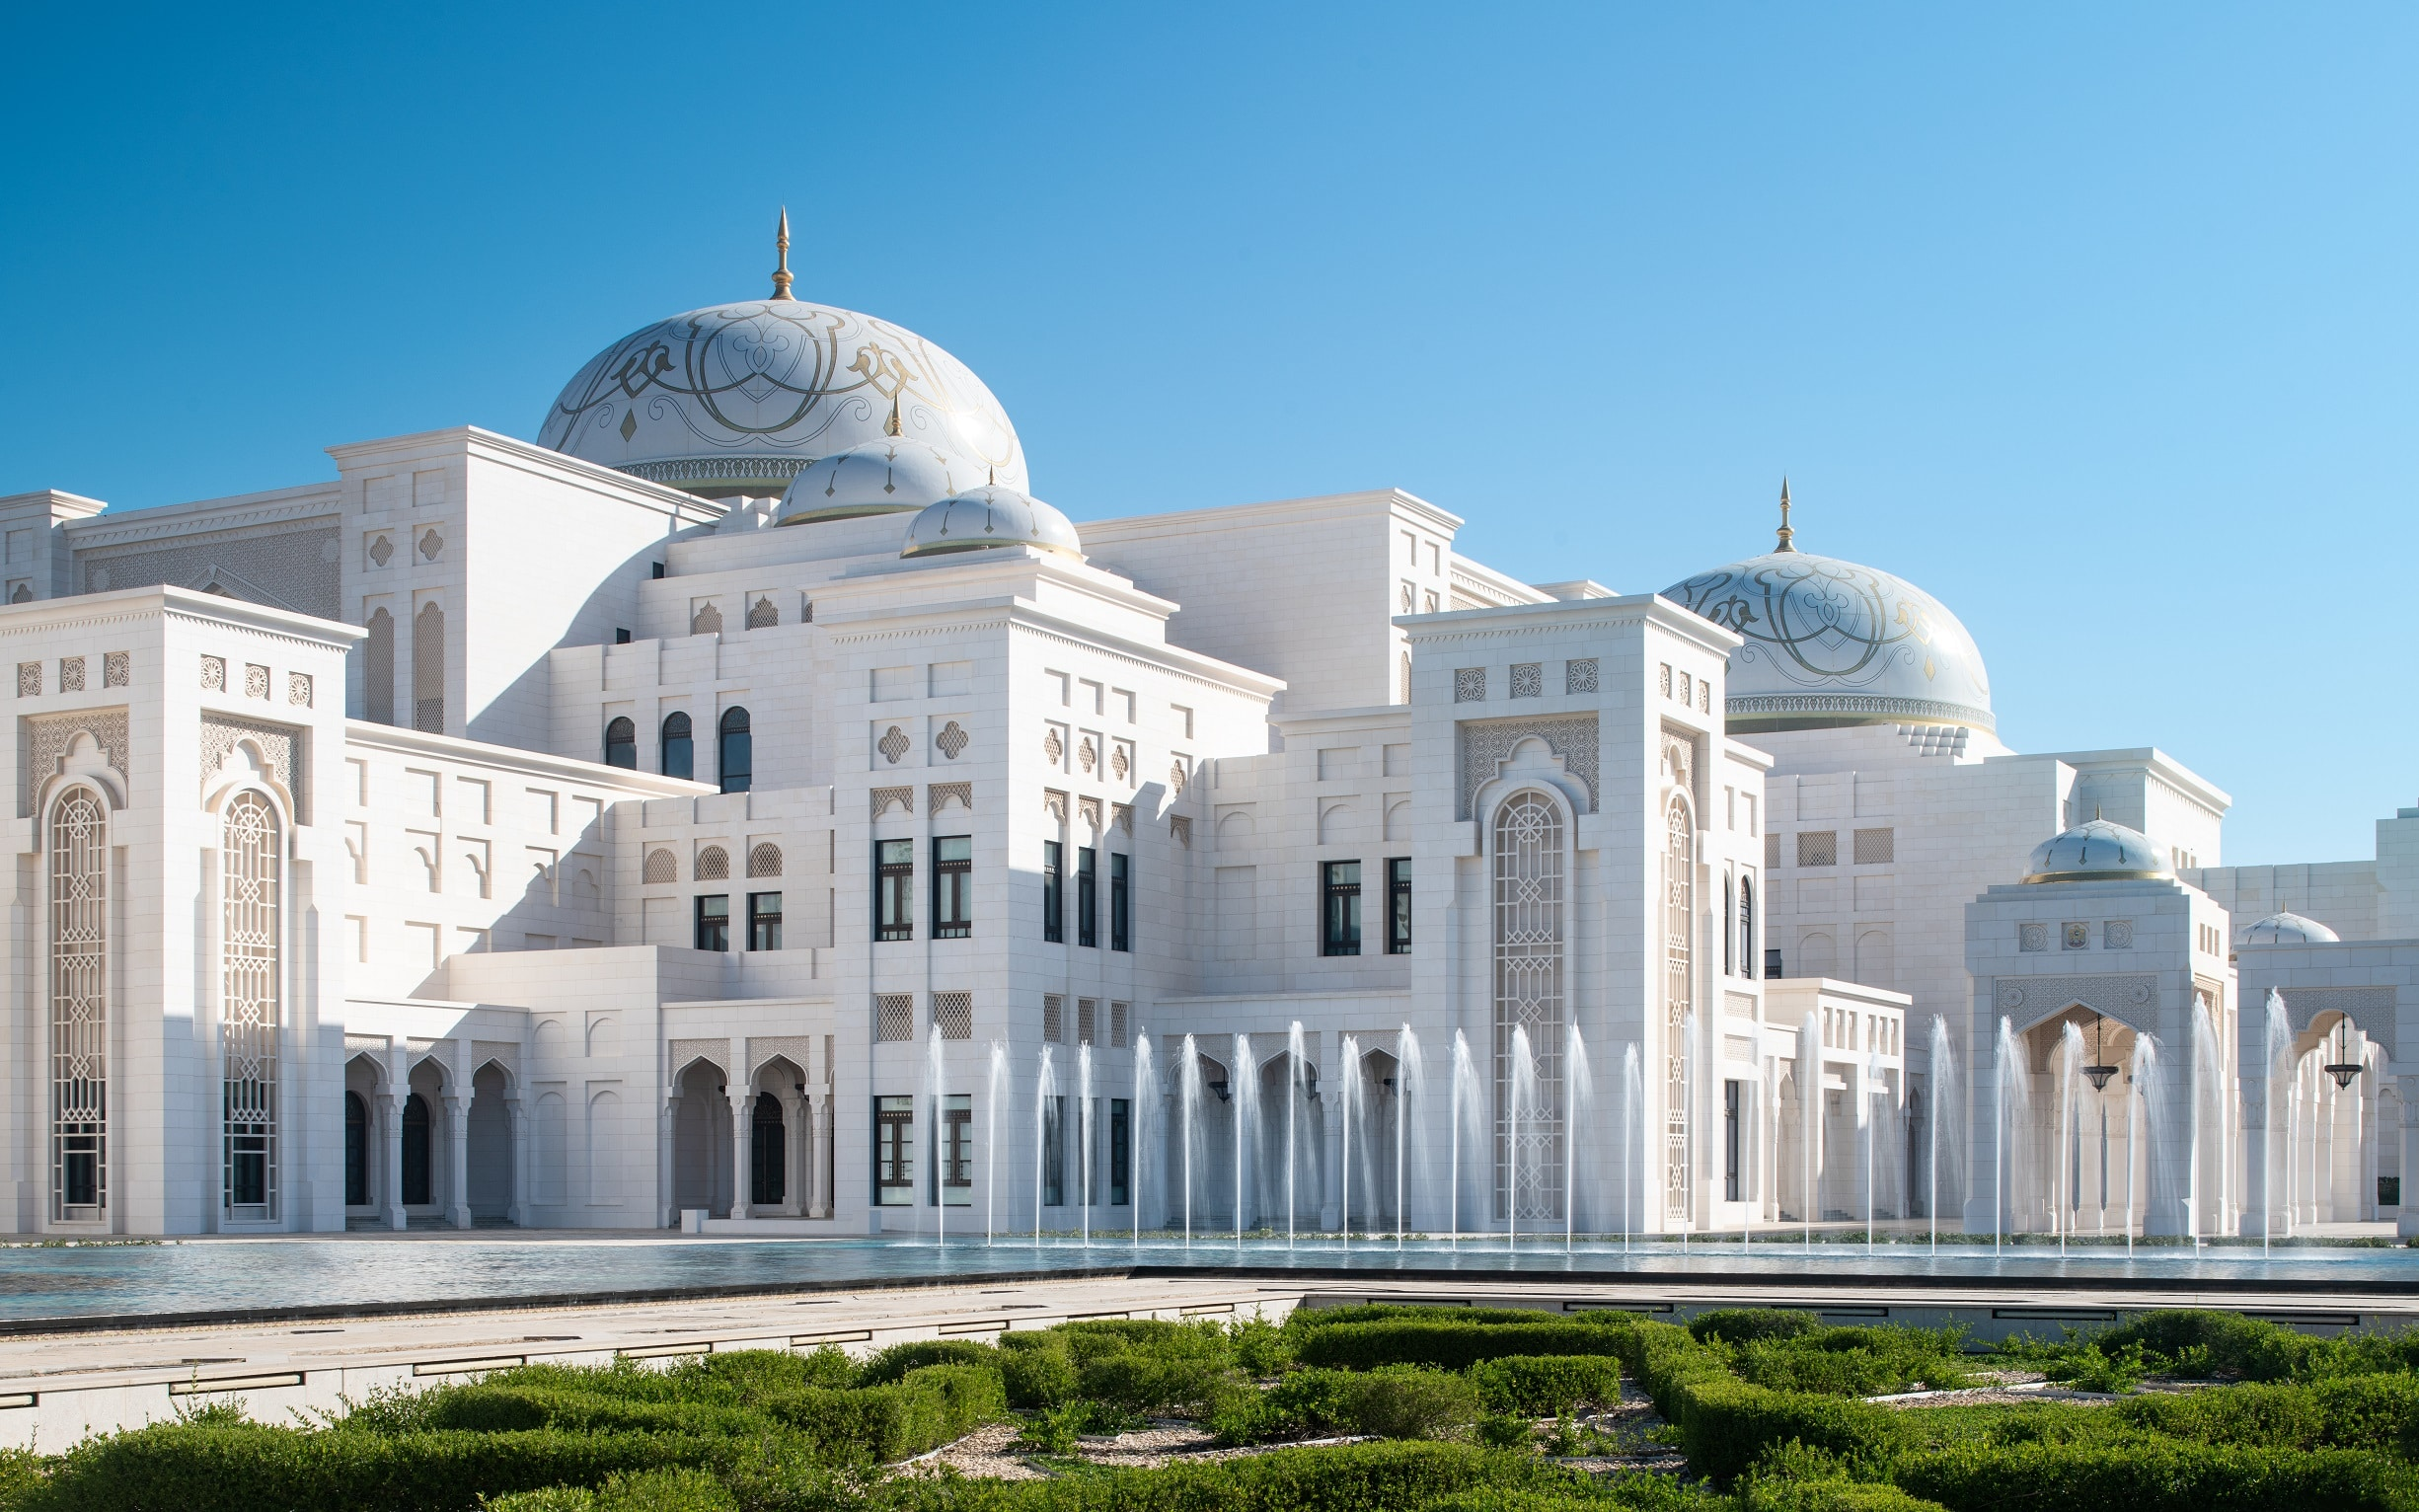
\includegraphics[width=0.45\linewidth]{examples/handbook_coling25/social_event/images/qasr_al-watan.png}
\end{figure}
\noindent{Next, the tour takes you to Qasr Al Watan, the presidential palace of the UAE. This magnificent palace showcases the rich culture and heritage of the Emirates. Visitors will tour the public areas, including the opulent Great Hall, stunning gardens, and exhibitions detailing the UAE’s history, governance, and future. The palace is an architectural and cultural wonder, with intricate designs and a breathtaking central dome that is among the largest in the world.}\\
\noindent{Key highlights}
\begin{itemize}[noitemsep]
  \item Ornate designs and artwork reflecting UAE’s history
  \item Magnificent Great Hall with its impressive dome
  \item Beautifully landscaped gardens
  \item Insight into the leadership and vision of the UAE
\end{itemize}
\newpage
\subsection{Social Excursion Option 2: Abrahamic House and Louvre Abu Dhabi Afternoon Tour}
\noindent{\textbf{1. Abrahamic Family House}}\\
\begin{figure}[h!]
  \centering
      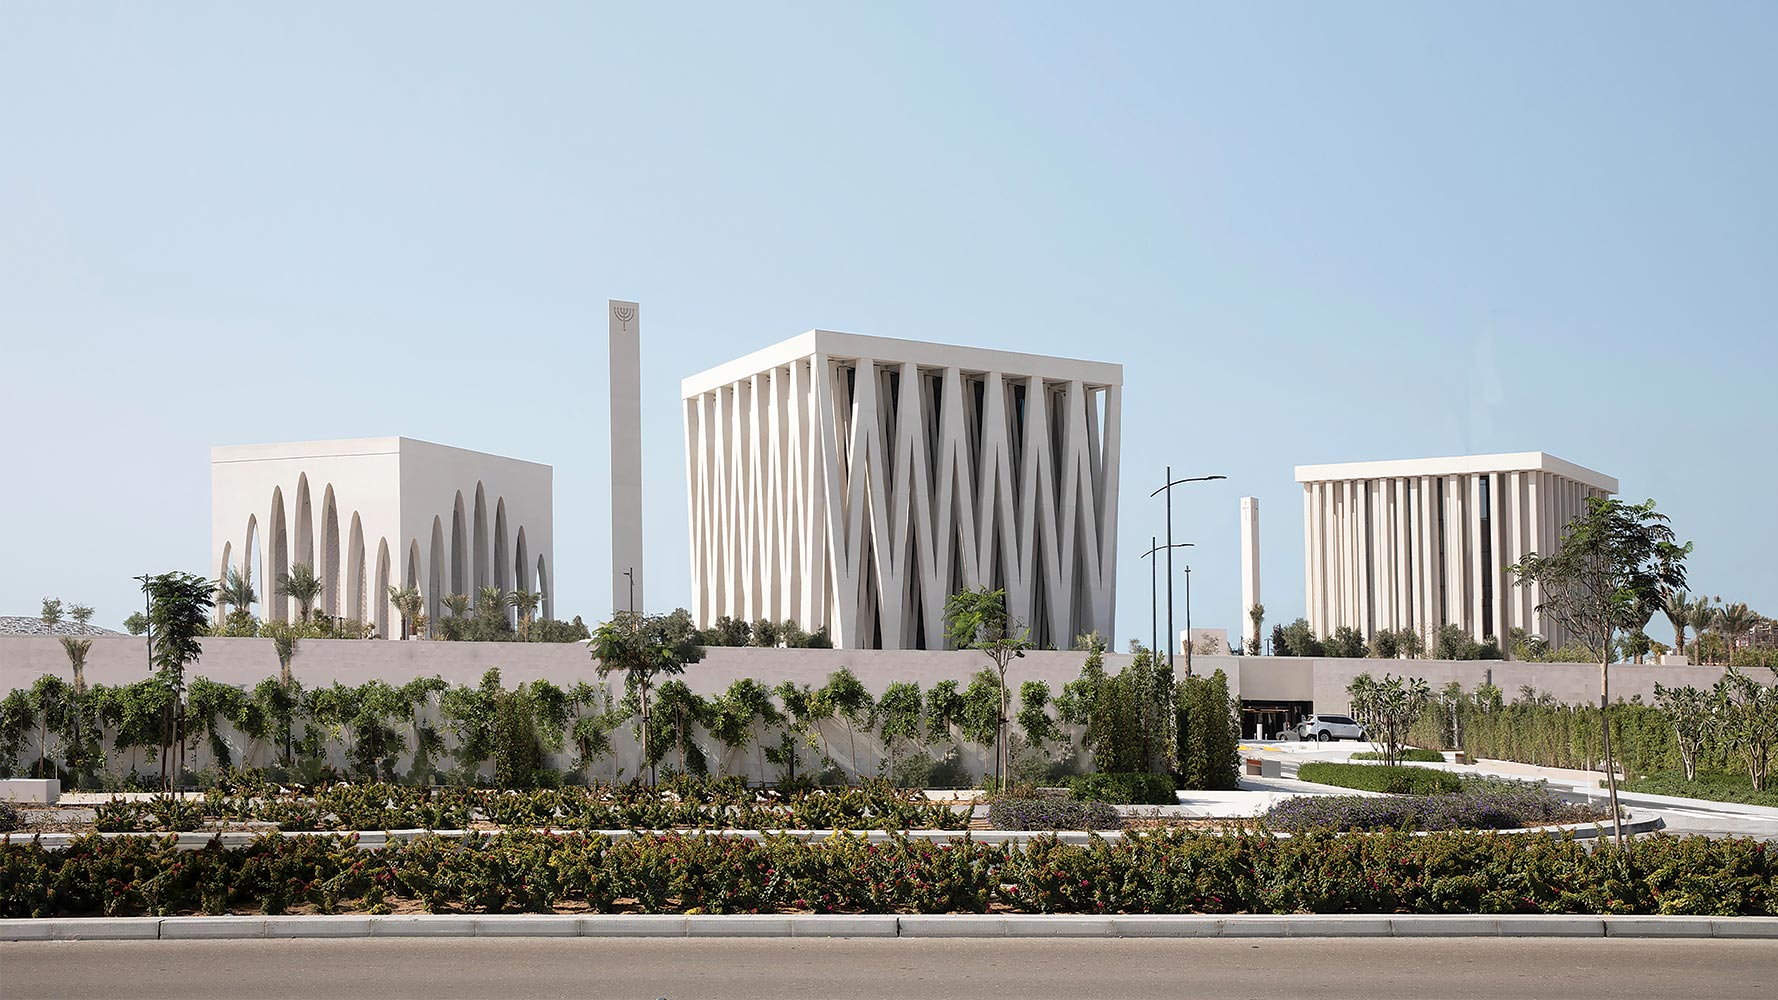
\includegraphics[width=0.45\linewidth]{examples/handbook_coling25/social_event/images/abrahamic_house.png}
\end{figure}
\noindent{The tour begins with a visit to the Abrahamic Family House, an iconic and historic complex that celebrates the shared values of the three Abrahamic religions: Islam, Christianity, and Judaism. Located on Saadiyat Island, this project is a symbol of peace, coexistence, and interfaith dialogue. The complex includes a mosque, a church, and a synagogue, each designed with stunning architecture that reflects the individual traditions while promoting unity. Visitors can explore the grounds, learn about the spiritual significance of each building, and appreciate the messages of tolerance and mutual respect.}\\
\noindent{Key highlights}
\begin{itemize}[noitemsep]
  \item Explore the mosque, church, and synagogue, each with unique architectural styles.
  \item Learn about the interfaith dialogue and the cultural importance of religious unity.
  \item Reflect on the harmonious message of the Abrahamic religions.
\end{itemize}
\noindent{\textbf{2. Louvre Abu Dhabi}}\\
\begin{figure}[h!]
  \centering
      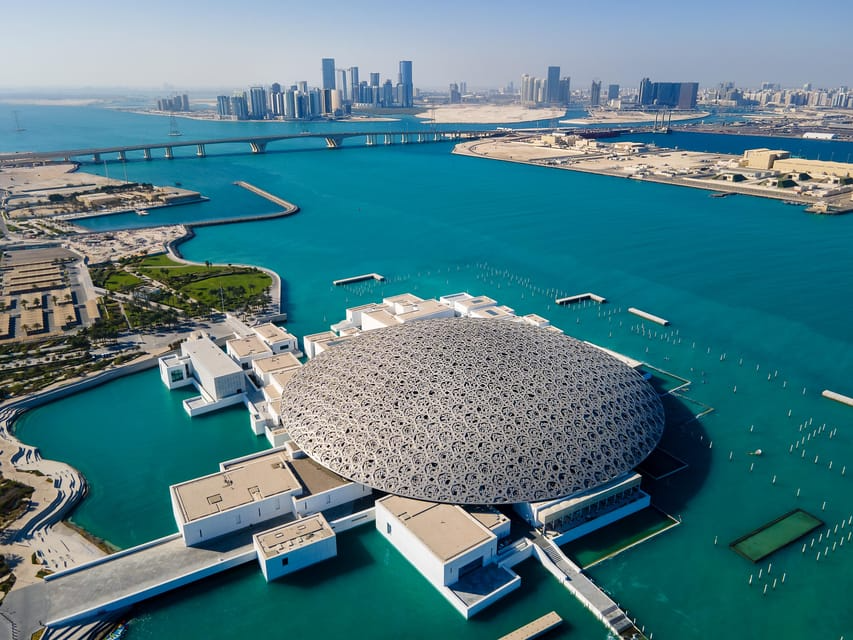
\includegraphics[width=0.45\linewidth]{examples/handbook_coling25/social_event/images/Louvre_AD.png}
\end{figure}
\noindent{Next, you’ll visit the Louvre Abu Dhabi, one of the most famous museums in the region. Located on Saadiyat Island, this museum is a cultural beacon showcasing art, history, and civilizations from across the globe. The museum is renowned for its stunning architecture, including a massive dome that creates a mesmerizing light effect, often referred to as the “rain of light.” Inside, the Louvre displays a vast collection of artworks from ancient civilizations to contemporary pieces, including paintings, sculptures, and artifacts from various cultures and time periods. The museum promotes cultural exchange and the sharing of human heritage.}\\
\noindent{Key highlights}
\begin{itemize}[noitemsep]
  \item A breathtaking collection of art and artifacts spanning different cultures and epochs.
  \item The iconic dome and the “rain of light” effect.
  \item Masterpieces from renowned artists such as Leonardo da Vinci, Van Gogh, and Monet.
  \item Rotating exhibits and installations that celebrate global heritage.
\end{itemize}
\newpage
\subsection{Social Excursion Options 3: Sand Dunes \& 4x4 Desert Safari}
\noindent{\textbf{1. Sand Dunes \& 4x4 Desert Safari}}\\
\begin{figure}[h!]
  \centering
      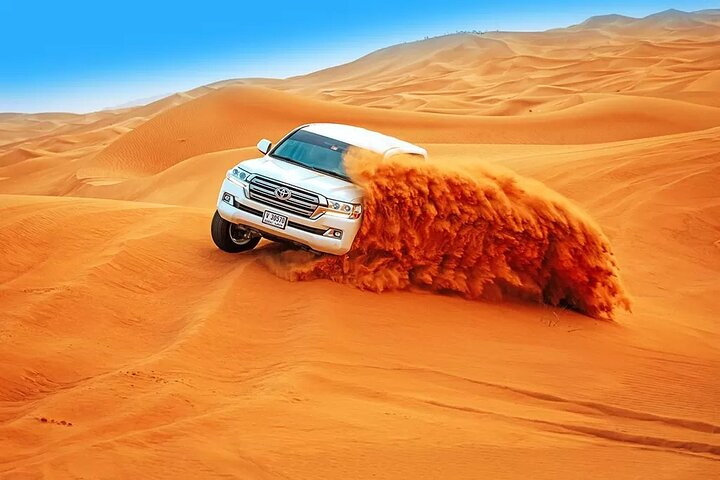
\includegraphics[width=0.45\linewidth]{examples/handbook_coling25/social_event/images/dune_bashing.png}
\end{figure}
\noindent{The tour begins with an exciting 4x4 desert safari as guests are driven into the vast, golden dunes of the Abu Dhabi desert. The ride is thrilling, with expert drivers navigating the towering sand dunes, providing a mix of dune bashing and scenic views. As you travel deeper into the desert, you’ll have the chance to experience the striking beauty of the undulating sand dunes, which stretch as far as the eye can see.}\\
\noindent{Key highlights}
\begin{itemize}[noitemsep]
  \item Exciting dune bashing in a 4x4 vehicle.
  \item Stunning views of the vast desert landscape.
  \item Thrill of riding over high dunes and through valleys.
\end{itemize}
\noindent{\textbf{2. Camel Riding}}\\
\begin{figure}[h!]
  \centering
      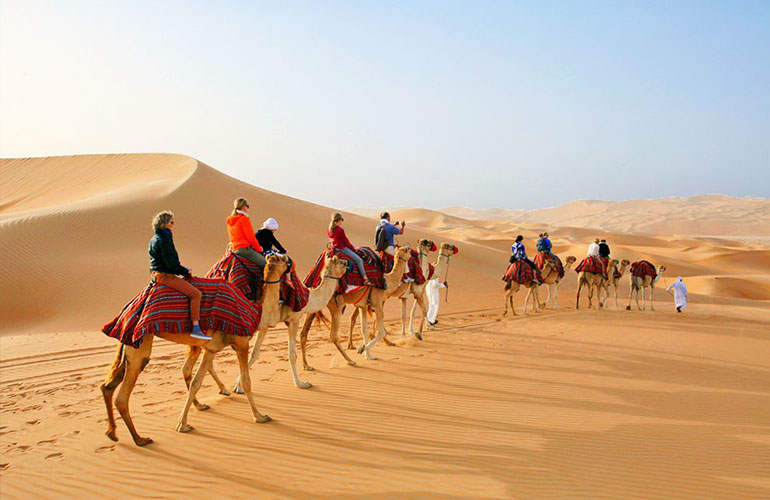
\includegraphics[width=0.45\linewidth]{examples/handbook_coling25/social_event/images/camel-trekking.png}
\end{figure}
\noindent{Next, you’ll experience a more traditional desert mode of transport with a camel ride. Camels, known as the “ships of the desert,” offer a unique and relaxing way to explore the landscape. As you gently sway atop the camel’s back, you’ll feel transported to an earlier time when camels were the main means of crossing the desert.}\\
\noindent{Key highlights}
\begin{itemize}[noitemsep]
  \item Enjoy a camel ride through the dunes, offering a slower-paced experience.
  \item Capture stunning desert scenery from the back of the camel.
  \item Learn about the cultural significance of camels in Bedouin life.
\end{itemize}
\noindent{\textbf{3. Sand Surfing}}\\
\begin{figure}[h!]
  \centering
      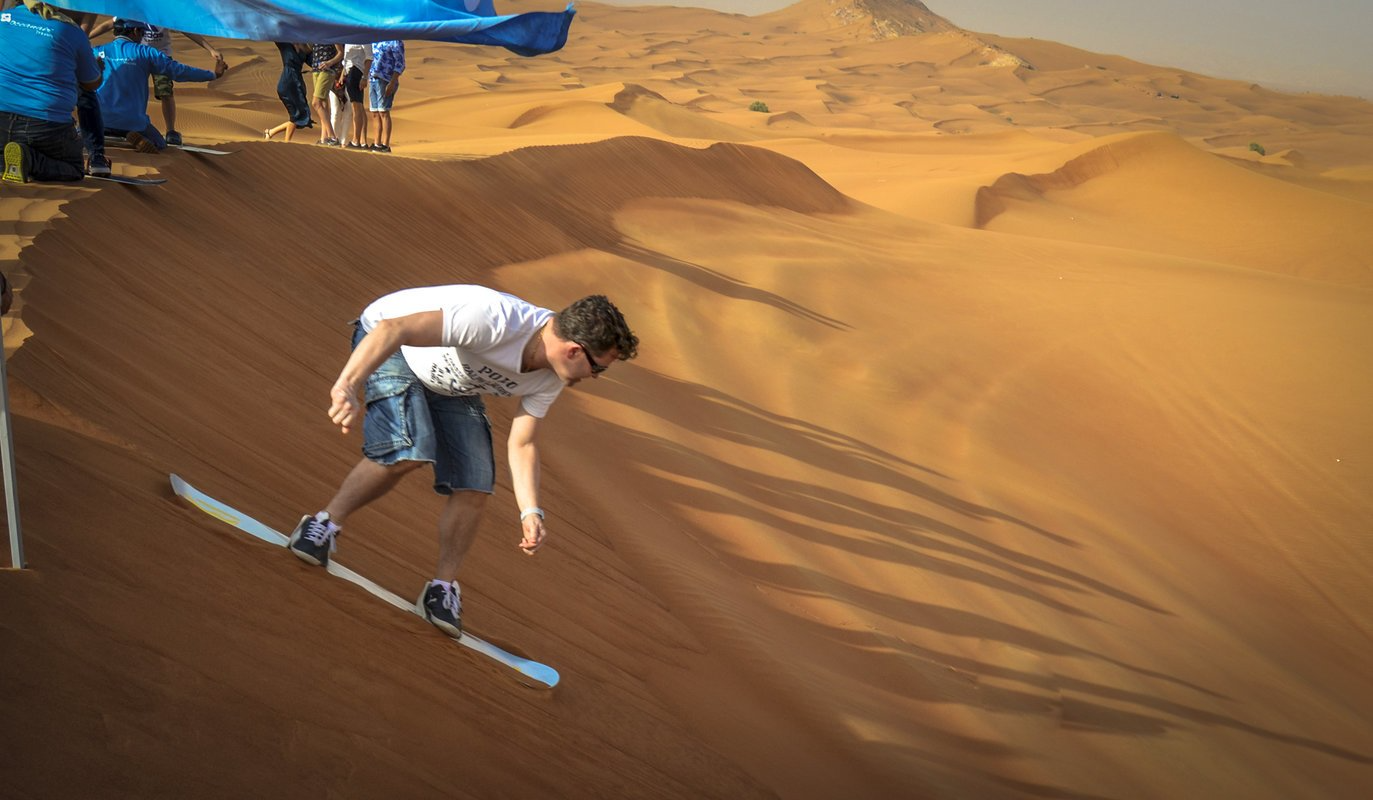
\includegraphics[width=0.45\linewidth]{examples/handbook_coling25/social_event/images/sand_surfing.png}
\end{figure}
\noindent{For an additional adrenaline rush, the tour includes the opportunity to try sand surfing. You’ll receive a sandboard and be guided to the perfect dune where you can attempt to glide down the sand slopes. Whether you’re an experienced surfer or a beginner, the thrill of gliding down the desert dunes is a unique and exhilarating experience.}\\
\noindent{Key highlights}
\begin{itemize}[noitemsep]
  \item Sand surfing down the dunes for a fun adventure.
  \item Experience the sensation of surfing on soft, golden sand.
  \item Great for both beginners and those looking for a challenge.
\end{itemize}
\noindent\hrulefill

\noindent{ \textbf{Boxed Lunch}}
\noindent{As part of the tour, guests will enjoy a boxed lunch perfect for a quick and convenient meal between sightseeing stops.}\\

\noindent{\textbf{Transport \& Convenience}}
\noindent{The tour includes bus transfers, ensuring a smooth and comfortable journey between each destination, allowing guests to focus on enjoying the experience without worrying about logistics.}\\

\noindent{\textbf{Dinner}}
\noindent{All Social Excursions meet up in the Desert for dinner under the Stars.
As the evening sets in, the adventure transitions to the serene desert landscape. The experience includes a traditional desert camp, where a lavish dinner awaits under the starlit sky. The dinner spread includes a BBQ buffet of local and international dishes, from grilled meats to vegetarian options, along with dessert and refreshing drinks.}\\

\noindent{\textbf{Entertainment}}
\noindent{As you enjoy your meal, the evening is further enhanced by live entertainment. Guests will be treated to a variety of traditional performances, including belly dancing, the colorful tanoura dance, and Arabic music, all contributing to the cultural atmosphere of the desert camp. The lively performances add to the enchantment of dining under the stars.}
\newpage
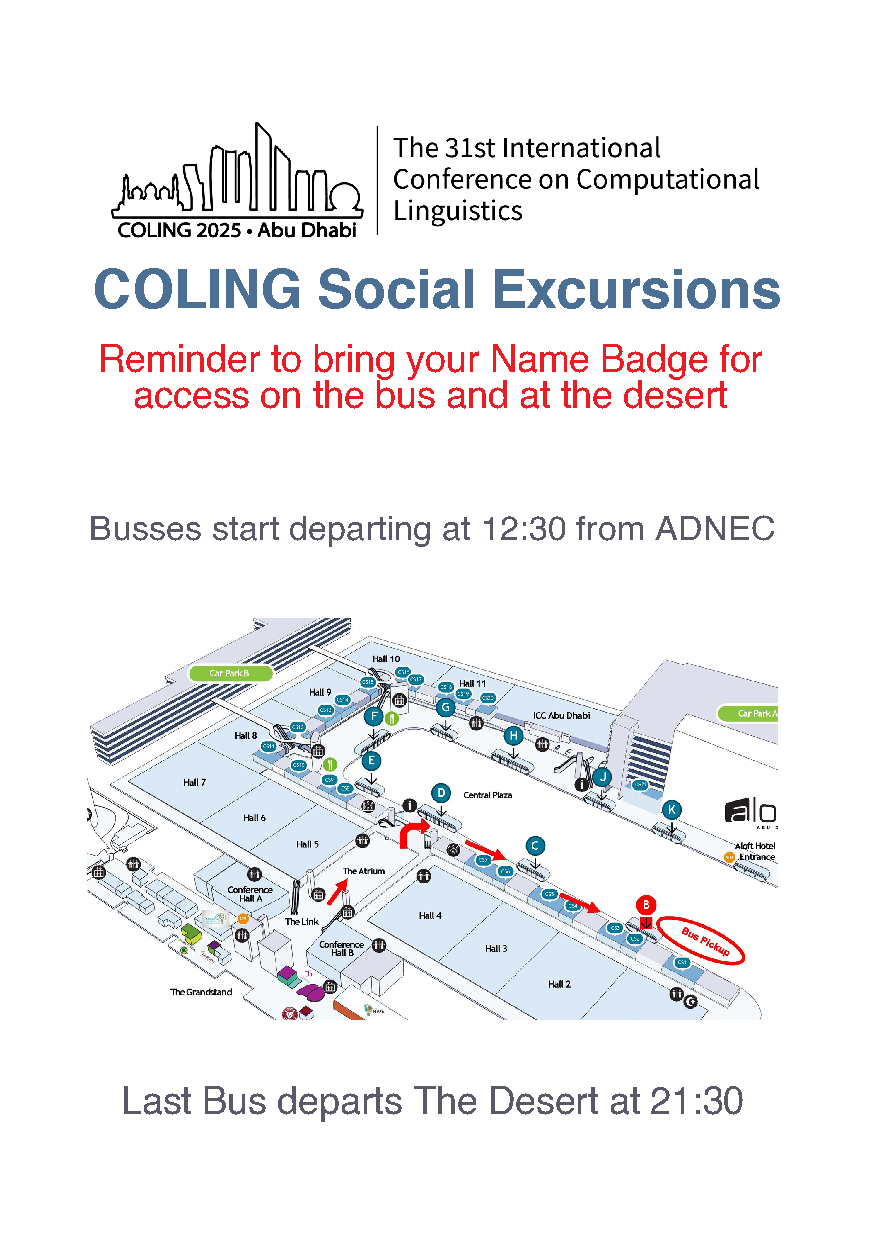
\includepdf[pages=-]{examples/handbook_coling25/social_event/Excursion_Map_for_Bus.pdf}